% Fig. 2 of the MLSP paper (figures/iid_grid.pdf).  The paper shows the
% four panels in one wide strip; on an A4 page the strip is split, as on
% the poster, into the legend, the P_d-versus-n pair and the rho-sweep pair
% (the trim values crop the single PDF).
\begin{figure}[htbp]
\centering
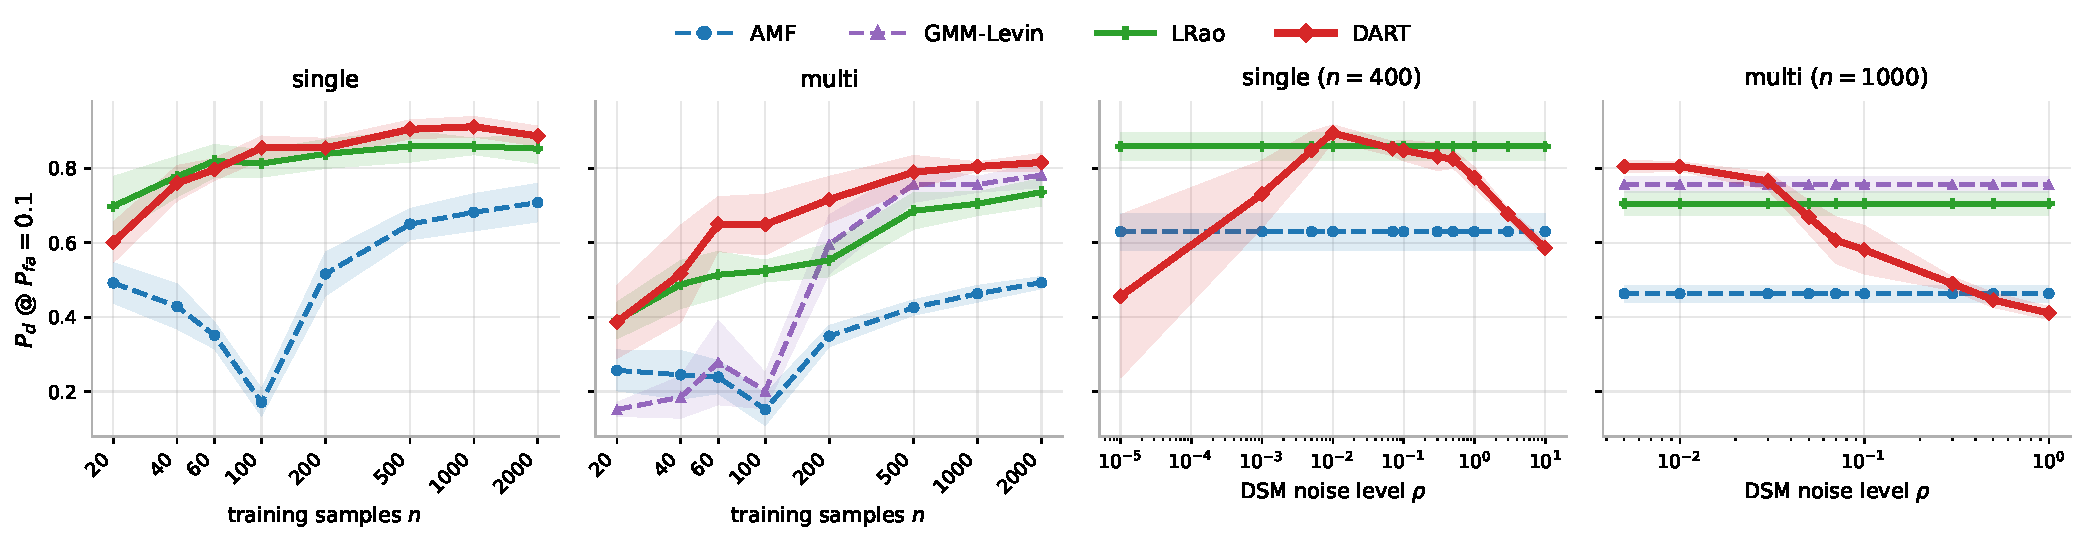
\includegraphics[width=0.55\textwidth, trim=322 238.8 322 9, clip]{figures/iid_grid.pdf}\\[2mm]
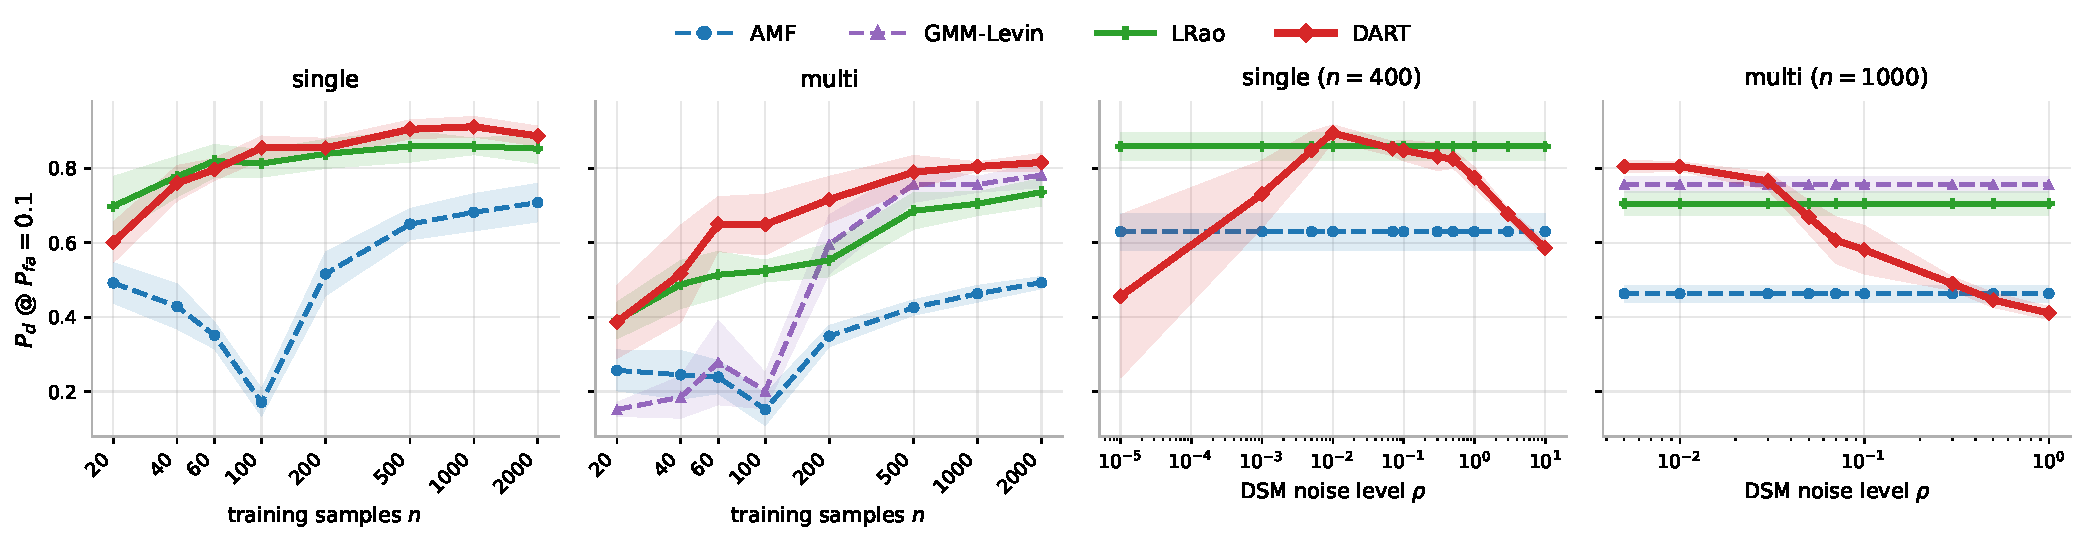
\includegraphics[width=\textwidth, trim=4.8 5.6 487.4 30.4, clip]{figures/iid_grid.pdf}\\[3mm]
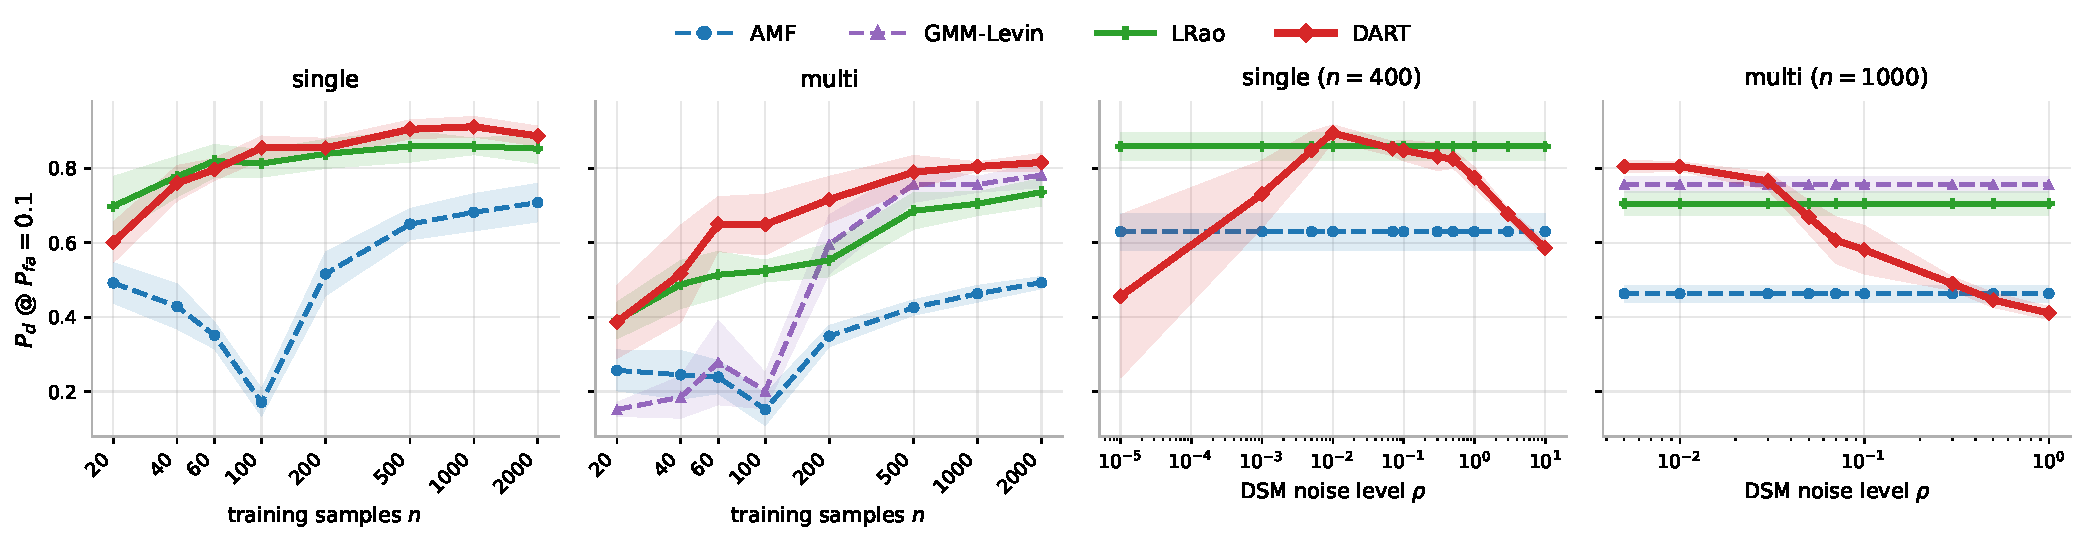
\includegraphics[width=\textwidth, trim=517 5.6 2 30.4, clip]{figures/iid_grid.pdf}
\caption{IID experiments on Pavia University ($5$ seeds, $\pm1\sigma$
bands). \emph{Top row}: $P_d$ at $P_{fa}=0.1$ versus the number of
secondary samples $n$ for the single-class and multi-class backgrounds;
the unregularized AMF collapses near $n\approx d$, where the sample
covariance is rank deficient, whereas the learned detectors are unaffected;
for DART this stability comes from the implicit loading supplied by the DSM
noise. \emph{Bottom row}:
robustness to the DSM noise level $\rho$ at fixed $n$. On the single-class
background, performance is flat over a wide plateau spanning
$\rho\in[5\!\times\!10^{-3},5\!\times\!10^{-1}]$; on the multi-class
background it peaks at small $\rho$ and degrades monotonically as the
blur washes out the mixture structure DART exploits. The operating point
$\rho=0.01$, used in the IID experiments, sits at the optimum in
both cases ($\rho$-independent detectors are drawn as flat references).}
\label{fig:ablation_single}
\label{fig:ablation_multi}
\end{figure}
